\documentclass[10pt,twoside,twocolumn]{article}
\usepackage[bg-letter]{dnd} % Options: bg-a4, bg-letter, bg-full, bg-print, bg-none.
\usepackage[ngerman]{babel} % Trennungsregeln und autom. Überschriften in n. dt. RS
\usepackage[utf8]{inputenc}
\usepackage{graphicx}
\usepackage{color}
\graphicspath{ {img/} }

% Start document
\begin{document}
\fontfamily{ppl}\selectfont % Set text font

% Your content goes here

\section{Introduction}
Ultimately the study of physiology is the study of "how stuff works." Physiology is primarily concerned with function. Often the terms Anatomy and Physiology are found together as a common phrase. Anatomy is the basic science of naming structures, and is an important component of physiological study, as we cannot describe function without a common scientific vocabulary provided by anatomy. But while anatomy is a study of rote memorization, physiology is a dynamic and process-based way of looking at how organisms function, from cell to tissue to organ to systems. The overall stability inherent in the functioning system is often a fascinating emergent property that can only be viewed with a thorough understanding of how the individual components work on their own, and then how they are integrated to generate a whole that is greater than the sum of its parts. 

The goal of this course is to give the student a basic understanding of the combined interaction of the major mammalian organ systems. It is taught with the common backdrop of homeostasis as a guiding principle, with an emphasis on how the nervous system integrates function across multiple systems. 

\subsection{HOMEOSTASIS}
% use \subsubsection{TEXT} for further organization of these sections
\textbf{Homeostasis} is the property of a system in which a given physiological variable is actively regulated in such a way as to remain close to a give \textit{set point} for that variable. 
\begin{commentbox}{The History of the term "Homeostasis"}
	Walter Cannon developed the concept of homeostasis from an earlier idea put forth by French Scientist Claude Bernard of \textit{milieu interieur}, and published it in his book \textit{The Wisdom of the Body} in 1932. Cannon presented four propositions to describe the general features of homeostasis:
    \begin{enumerate}
\item Constancy in an open system, such as our bodies represent, requires mechanisms that act to maintain this constancy. 
\item Steady-state conditions require that any tendency toward change automatically meets with factors that resist change. 
\item The regulating system that determines the homeostatic state consists of a number of cooperating mechanisms acting simultaneously or successively. 
\item Homeostasis does not occur by chance, but is the result of organized self-government.
\end{enumerate}
\end{commentbox}

\begin{quotebox}
	\textbf{A note on the generation, editing, and use of this document.} This is the first version of a class-drive communal "textbook"  for this course. All are welcome to add to, edit, or otherwise improve the document. However, final version control rests with the Instructor. Because this is an open-source document, it should not be assumed that the Instructor will be able to verify the contents continuously. Therefore, there is no substitute for your own notes and attendance of class. This text is \underline{NOT} valid as the sole resource for disputes regarding grades or test answers. 
\end{quotebox}

%\newpage % Acts as columnbreak because of twocolumn option; for pagebreak use \clearpage

\begin{dndtable}{XX} % XX defines there will be two columns, add more to get more columns
   	\textbf{Physiological Variable}  & \textbf{Systems Involved} \\
   	????  & ???? \\
   	????  & ???? \\
   	????  & ????
\end{dndtable}

Most common physiological variables are maintained within a predictable range, despite potentially wildly changing external environments. \textbf{Homeostasis} is the process by which these variables are maintained. It is this reliable internal environment that is optimal for cell function that is largely the entire reason that complex organs, systems, and organisms exist; to provide the optimal environment for cell survival and replication. Yet there is no such thing as a physiological variable that is maintained at a true constant value over time.  Rather, homeostasis is a dynamic process that aims for a predictable \textit{time-averaged mean} for a variable rather than an invariant steady state.  

\subsection{CONTROL SYSTEMS}
\textcolor{red}{After the Lecture on Friday, January 20, we will add content here regarding set points, negative feedback loops, integrating centers, and all that good stuff.  Please feel free to add content here.}

\clearpage

\begin{paperbox}{RESEARCH FOCUS: WHAT IS CELL CULTURE?}
"Cell culture is the process by which cells are grown under controlled conditions, generally outside of their natural environment. Cell culture conditions can vary for each cell type, but artificial environments consist of a suitable vessel with substrate or medium that supplies the essential nutrients (amino acids, carbohydrates, vitamins, minerals), growth factors, hormones, and gases (CO$_2$, O$_2$), and regulates the physio-chemical environment (pH buffer, osmotic pressure, temperature). Most cells require a surface or an artificial substrate (adherent or monolayer culture) whereas others can be grown free floating in culture medium (suspension culture).

In practice, the term generic term 'cell culture' most often refers to  culturing of cells derived from multicellular eukaryotes, especially animal cells, in contrast with other types of culture that also grow cells, such as plant tissue culture, fungal culture, and microbial culture. The historical development and methods of cell culture are closely interrelated to those of tissue culture and organ culture." (Source: Wikipedia)
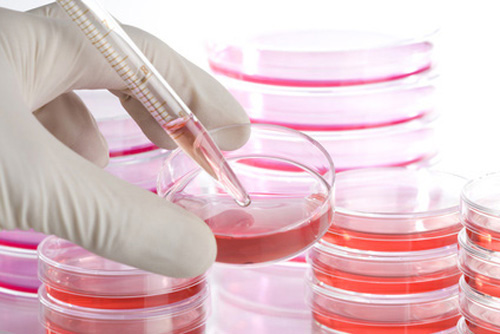
\includegraphics[width=\textwidth]{CElCulture.jpg}
[Sven Hoppe - Fotolia.com]
\end{paperbox}

\subsection{TISSUE TYPES}
While biological classification can always be further subdivided along a continuum, in general we will consider four major tissue types as the major constituents of organs and organ systems.  A \textbf{Tissue} is defines as \textit{a group of similar cells, usually from the same developmental origin, that work together to carry out a specific function}. \textbf{Organs} are then formed from the grouping together of multiple tissue types.

The four major tissue types are as follows:
	\begin{enumerate}
	\item \textbf{Epithelial}: [please add content here]
    \item \textbf{Connective}: [please add content here]
    \item \textbf{Nervous}: [please add content here]
    \item \textbf{Muscle}: [please add content here]
    \end{enumerate}



% End document
\end{document}
